\section{Multiple testing and differential gene expression}
\label{FDR}

We present an experiment involving Bayesian hypothesis testing for detecting differentially expressed genes from single-cell transcriptomics data, a central problem in modern molecular biology. Single-cell RNA sequencing data (scRNA-seq) provides a noisy snapshot of the gene expression levels of cells~\cite{Wagner2016, Tanay2017}. It can reveal cell types and gene markers for each cell type as long as we have an accurate noise model~\cite{Grun2014}. scRNA-seq data is a cell-by-gene matrix $X$.
For cell $n=1,\ldots,N$ and gene $g=1,\ldots,G$,
entry $X_{ng}$ is the number of transcripts for gene $g$ observed in cell $n$.
Here we take as given that each cell comes paired with an observed cell-type label $c_n$. 

Single-cell Variational Inference (scVI)~\cite{Lopez292037} is a hierarchical Bayes model~\cite{GelmanHill:2007} for scRNA-seq data. For our purposes here, it suffices to know that the latent variables $h_{ng}$ represent the underlying gene expression level for gene $g$ in cell $n$, corrected for a certain number of technical variations (e.g., sequencing depth effects). The corrected expression levels $h_{ng}$ are more reflective of the real proportion of gene expression than the raw data $X$~\cite{Cole2017}. Log-fold changes based on $h_{ng}$ can be used to detect differential expression (DE) of gene $g$ across cell types $a$ and $b$~\cite{deseq2,Boyeau794289}. Indeed, Bayesian decision theory helps decide between a model of the world $\mathcal{M}_1^g$ in which gene $g$ is DE and an alternative model $\mathcal{M}_0^g$ of non-DE. The hypotheses for the Bayesian hypothesis testing problem we are interested in are
\begin{align}
    \mathcal{M}^g_1: \left|\log\frac{h_{ag}}{h_{bg}}\right| \geq \delta ~~~~ \text{and}~~~ \mathcal{M}^g_0: \left|\log\frac{h_{ag}}{h_{bg}}\right| < \delta,
    \label{hypotheses}
\end{align}
where $\delta$ is a threshold defined by the practitioner. DE can therefore be performed by posterior estimation of log-fold change between two cells $x_a, x_b$, which can be written as
\(
p_\theta(\mathcal{M}^g_1 \mid x_a, x_b)
\)
% \begin{align}
% \label{eq_de_probability}
%   \begin{split}
%     & p_\theta \left( 
% \left|\log\frac{h_{ag}}{h_{bg}} \right| \geq \delta
% \mid x_a, x_b 
% \right),
%     \end{split}
% \end{align}
and estimated with importance sampling.
The optimal decision rule for 0-1 loss is attained by thresholding the posterior log-fold change estimate.
Rather than directly setting this threshold, a practitioner typically picks a false discovery rate (FDR) $f_0$ to target. For controlling the FDR, 
we consider the multiple binary decision rule $\mu^k = (\mu_g^k, g \in G)$ that consists of tagging DE the $k$ genes with the highest posterior estimate of log-fold change.
With this notation, the false discovery proportion (FDP) of such a decision rule is
\begin{align}
    \mathrm{FDP} = 
        \frac
        {\sum_g (1 - \mathcal{M}_1^g) \mu_g^k}
        {\sum_g \mu_g^k}.
\end{align}
Following~\cite{Cui2015}, we define the posterior expected FDR as
\(
\overline{\mathrm{FDR}} := \mathbb{E}\left[\mathrm{FDP} \mid x_a, x_b\right],
\)
% \begin{align}
%     \overline{\mathrm{FDR}} :=     
%     \mathbb{E}
%     \left[ 
%     \frac
%     {\sum_g (1 - d^g) \mu_g^k}
%     {\sum_g \mu_g^k} 
%     \mid x_a, x_b \right],
%     \label{FDR_estimate}
% \end{align}
which can be computed from the differential expression probabilities of Eq.~\eqref{hypotheses}. We then set $k$ so that it is the maximum value for which the posterior expected FDR is below $f_0$. 
In this case, controlling the FDR requires estimating $G$ posterior expectations. % We denote by $\bar{\mu}$ the decision rule associated with the threshold $0.10$.
To quantify the success of a given method at controlling the FDR at any arbitrary level, we will report the mean absolute error between the groundtruth FDR and the posterior expected FDR. 

\begin{figure}
\centering
\captionsetup{type=table}
\begin{center}
\begin{small}
\begin{tabular}{lccccccc}
\toprule
 & \textbf{VAE}  & \textbf{IWAE} & \textbf{WW} & \textbf{$\chi$-VAE} \\ \midrule
 AIS & -379.93 & \textbf{-375.53} & -376.34 & -376.66 \\
IWELBO  & -381.50 & \textbf{-376.21} & -377.01 & -378.32\\
\midrule
PSIS  & \textbf{0.67} & 0.73 & 0.86 & 0.76\\
\midrule
MAE FDR & 8.49 & \textbf{0.97} & 1.10 & 1.52 \\
\bottomrule
\end{tabular}
\end{small}
\end{center}
\caption
[Results for the scVI model]{\label{table_fdr}
Results for the scVI model. MAE FDR refers to the mean absolute error for FDR estimation.}

\end{figure}

\begin{figure}
\centering
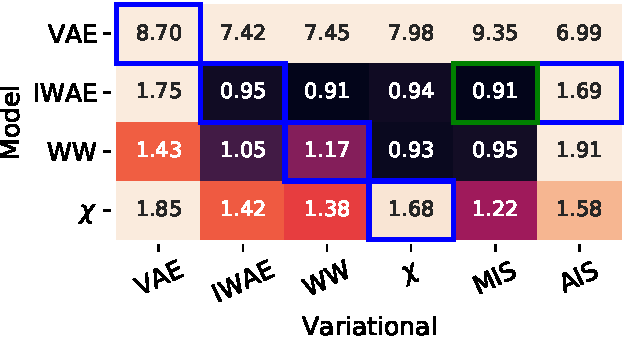
\includegraphics[width=0.4\textwidth]{figures/fdr_l1_err_cross.pdf}
\caption[MAE FDR for scVI]{MAE FDR for scVI: combinations of VAEs (row) and inference only (columns) frameworks. }\label{fig:scVI-cross}
\end{figure}

We fit the scVI model with all the objective functions of interest. In addition, we also use annealed importance sampling (AIS)~\cite{neal2001annealed} to approximate the posterior distribution once the model is fitted. AIS is computationally intensive, so we used $500$ steps and $100$ samples from the prior to keep a reasonable runtime. Because the ground-truth FDR cannot be computed on real data, we generated scRNA-seq data according to a Poisson Log-Normal model (a popular choice for simulating scRNA-seq data~\cite{townes2019feature,Crowell713412}) from five distinct cells types corresponding to $10,000$ cells and $100$ genes. This model is meant to reflect both biological signal and technicalities of the experimental protocol. % SymSim~\cite{zhang2019simulating}. SymSim is a simulator that draws measurements from a Beta-Poisson marginal distribution for each cell and gene and adds technical noise by downsampling to reflect both biological signal and technicalities of the experimental protocol. We generated count data 


VAE performs worse in terms of held-out log-likelihood (both IWELBO and AIS), while IWAE performs best (Table~\ref{table_fdr}). We also evaluate the quality of the gene ranking for differential expression, based on the AUPRC of the DE probabilities. The model learned with the VAE objective function has an AUPRC of 0.85 while all other combinations have an AUPRC of more than 0.95. Next, we investigate the role posterior uncertainty plays in properly estimating the FDR.  
Table \ref{table_fdr} and Figure~\ref{fig:scVI-cross} report the mean absolute error (MAE) for FDR estimation over the 100 genes. The posterior expected FDR has a large error for any proposal based on the VAE model (around 8\%, even worse using the plugin estimator). However, all other model yield a significantly lower error (from 1 to 2\%), for any proposal. 
We provided the PSIS and PRAUC in Figure~\ref{fig:XscVI-cross-other}, as well as the FDR curves and MAE estimates in Figure~\ref{fig:YscVI-cross-other}. The VAE has highly inaccurate FDR control while IWAE, WW and $\rchi$-VAE may be useful to a practitioner, also with some error. 
This suggests that the model learned by the original scVI training procedure (i.e., a VAE) cannot be used for FDR control, even using AIS to find a proposal. Conversely, our three-step procedure (IWAE-MIS) has the best FDR estimates on this experiment (a tie with IWAE-WW), improving over all the single-proposal alternatives as well as IWAE followed by AIS. %Finally, we noticed that running AIS after inference is much more computationally intensive ($14.5$ times longer per posterior evaluation) but does not provide substantial improvement. 


\begin{figure}
    \centering
    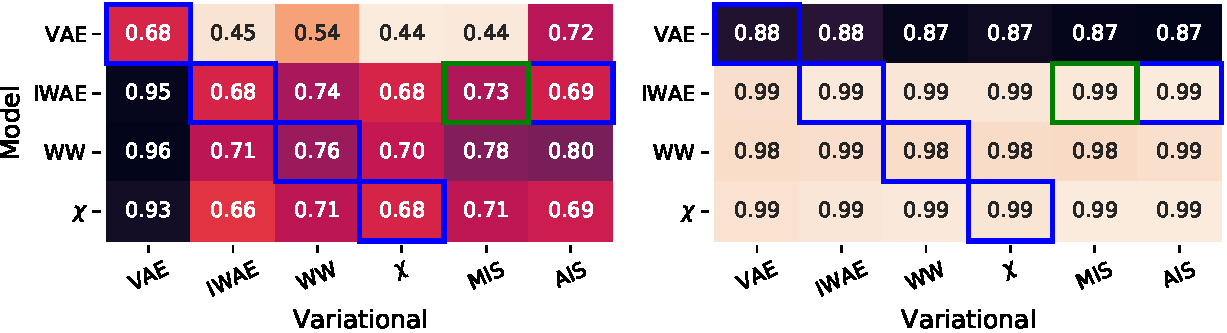
\includegraphics[width=0.65\textwidth]{figures/fdr_other_cross.pdf}
    \caption[PSIS and PRAUC for scVI]{
    PSIS (\textit{left}) and PRAUC (\textit{right}) for scVI: combinations of VAEs (row) and inference only (columns) frameworks. 
    }
    \label{fig:XscVI-cross-other}
\end{figure}


\begin{figure}
    \centering
    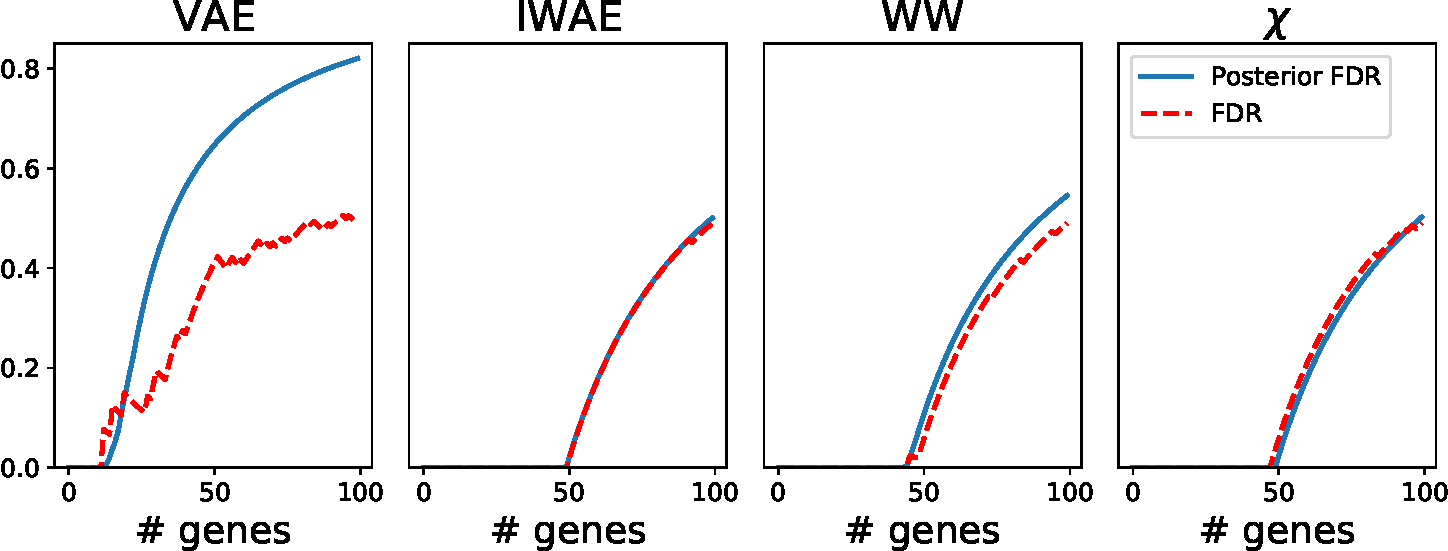
\includegraphics[width=0.7\textwidth]{figures/fdr_curves_gen.pdf}
    \caption[Posterior expected FDR and ground-truth FDR for the diferent models]{
    Posterior expected FDR (blue) and ground-truth FDR (red) of the decision rules consisting in selecting the genes with the highest DE probability for the different models.
    }
    \label{fig:YscVI-cross-other}
\end{figure}

